\documentclass[letterpaper]{article} % DO NOT CHANGE THIS
\usepackage[submission]{aaai2027}  % DO NOT CHANGE THIS
\usepackage[hyphens]{url}  % DO NOT CHANGE THIS
\usepackage{graphicx} % DO NOT CHANGE THIS
\urlstyle{rm} % DO NOT CHANGE THIS
\def\UrlFont{\rm}  % DO NOT CHANGE THIS
\usepackage{natbib}  % DO NOT CHANGE THIS AND DO NOT ADD ANY OPTIONS TO IT
\usepackage{caption} % DO NOT CHANGE THIS AND DO NOT ADD ANY OPTIONS TO IT
\frenchspacing  % DO NOT CHANGE THIS
\usepackage{booktabs}
\usepackage{amsmath}
\pdfinfo{
/TemplateVersion (2027.1)
}
\setcounter{secnumdepth}{0}

% Fallback version that fits in 4 pages INCLUDING references (in case the venue counts them).
% Same results and claims as main.tex; prose condensed, pilot table moved into text.

\title{Repair Without Regression? A Budget-Matched Audit of an Agent-Edited Robot Skill}
\author{
    Anonymous Submission
}
\affiliations{
}

\begin{document}

\maketitle

\begin{abstract}
When a coding agent edits a persistent robot controller to fix a failure, aggregate success can hide losses on scenes the controller used to solve. We test this in a fully controlled case: the scripted Franka pick-and-place controller in Isaac Sim, a measured-state evaluator, and a workspace-boundary failure found by documented search. The unchanged controller replays exactly, so every paired transition is caused by an edit. On the development panel, two frozen single-parameter repairs fixed the target and lost 4 and 1 of 44 earlier successes but gained more elsewhere, so aggregate and zero-loss admission disagreed. On a frozen audit of 160 fresh scenes this compensation did not replicate. Both repairs improved the target neighborhood (from 15/40 to 26/40 and 38/40) but lost 8 and 5 of 106 old successes against 4 gains each, and budget-matched aggregate and zero-loss gates both rejected both. In a post-hoc extension with 24 seeded random edits, all ten target-improving candidates lost old successes. On that fresh draw the two repairs' old net change turned positive, while their conditional loss rates replicated. The composition of the old-scene panel mattered more than the choice of admission rule.
\end{abstract}

\section{Introduction}
Coding agents increasingly improve robot behavior by editing executable controllers in response to simulated or real feedback \citep{kuroki2026closedloop,xiao2026enpire,aphale2026selfrepair}. When the edited artifact is a persistent skill, a repair made for one failure is carried into every later scene. The usual acceptance check---did success go up?---can hide a trade: the revised controller may solve new scenes while failing scenes it used to solve. Because the change in old-scene success equals gains minus losses, ``no aggregate decrease'' and ``no lost successes'' are different requirements. They differ only when a repair both breaks and fixes old scenes.

Whether that happens for robot skills, and how admission rules respond, has mostly been argued analytically or in software repair \citep{ma2026validation,gao2026looping}. We contribute a small, tightly controlled robot case study. It consists of a simulation setup in which the unchanged parent replays exactly, so each success-to-failure transition is caused by the edit; a development pilot in which aggregate and zero-loss admission disagreed; a frozen audit on 160 fresh scenes, with gate decisions committed before execution, in which they agreed; and a post-hoc population extension of 26 candidates and 3{,}800 rollouts. We do not propose a new verifier, learning algorithm or safety guarantee; regression testing and paired evaluation are established tools. The contribution is controlled evidence about directional gains and losses, and about when the choice of admission objective matters.

\section{Related Work}
Ma and Wu formalize update admission under evaluation budgets, including missed learning opportunities, with analytical and synthetic evaluation \citep{ma2026validation}; we study a simulated-robot instance of their question. Kuroki et al.\ refine closed-loop robot code with simulation feedback \citep{kuroki2026closedloop}, and ENPIRE runs an agentic improvement loop on real robots \citep{xiao2026enpire}. Aphale and Singh show that code-as-policy repair must be compared against resampling and static-guidance baselines \citep{aphale2026selfrepair}, so we make no claim about the proposer and hold candidates fixed across gates. In software agents, Gao et al.\ bind evidence to exact code states \citep{gao2026looping}, Xu and Wu test whether passing validation discriminates a fix \citep{xu2026evidence}, and Zhang et al.\ compare verification designs in agent harnesses \citep{zhang2026verification}. We adopt state-bound evidence and parent replay for a persistent robot skill.

\section{Setup}
\paragraph{Controller and evaluator.} We use Isaac Sim 6.2's scripted Franka pick-and-place controller \citep{nvidia2026franka} with CPU physics at 60\,Hz, one cube, a fixed place goal and an 1{,}800-step horizon. Edits are restricted to six bounded high-level parameters: approach height, lift height, motion and grasp convergence tolerances, stability duration and gripper dwell. Motion generation, scenes and the evaluator cannot be edited. Success $S(p,x)\in\{0,1\}$ for controller $p$ on scene $x$ is scored from simulator object state, independently of the controller's completion flag. The cube must be lifted above 7.58\,cm, and the episode must end before the horizon. Over 30 settling frames, the cube must stay within 3.0\,cm of the goal with the gripper more than 8\,cm away, linear speed below 0.02\,m/s, angular speed below 0.1\,rad/s and orientation drift below 0.05\,rad. Four negative controls---no motion, no grasp, holding at the goal, and a one-step timeout---are all rejected.

\paragraph{Directional outcomes.} For parent $p$, candidate $p'$ and old-scene distribution $D_o$, define
\begin{align*}
L &= \Pr\nolimits_{x\sim D_o}[S(p,x)=1,\; S(p',x)=0],\\
G &= \Pr\nolimits_{x\sim D_o}[S(p,x)=0,\; S(p',x)=1].
\end{align*}
Then $J_o(p')-J_o(p)=G-L$: an aggregate criterion constrains $G-L$, not $L$. If the parent solves every old scene, then $G=0$ and the two notions coincide; they come apart only when gains offset losses. We report the conditional loss $L/J_o(p)$ alongside $G$, $L$ and the target change.

\paragraph{Gates.} Every rule spends 24 rollouts per candidate; a pair is one parent and one candidate rollout on the same scene. \emph{Aggregate} uses 4 target and 8 old pairs and admits if the target net change is positive and the old net change is at least zero, given at least one parent old success. \emph{Preservation} uses the same pairs and also requires zero old losses. \emph{Target-only} uses 12 target pairs and admits if the target improves. \emph{Frozen} never admits. A rejected candidate leaves the parent deployed. No rule certifies safety: zero losses in eight draws is compatible with a substantial loss rate.

\paragraph{Failure discovery and repairs.} Development scenes were searched in documented, adaptive stages: twelve hand-specified scenes (36/36 successes); a radial grid of pick radii 0.35, 0.55 and 0.75\,m at angles from $-60^\circ$ to $60^\circ$ in $30^\circ$ steps (44/45); and a boundary ring at 0.80 and 0.85\,m (0/30). The first scene in manifest order that failed at least two of three resets became the target: radius 0.80\,m, angle $-60^\circ$. The cube is lifted, but the arm stalls in the lift phase with 2.0\,cm residual error against a 1.5\,cm convergence tolerance and times out. A coding assistant inspected the controller source and failure traces and proposed two single-parameter repairs, saved and hashed before execution. \textbf{A} lowers the lift height from 0.30 to 0.20\,m. \textbf{B} relaxes the motion convergence tolerance from 0.015 to 0.025\,m, leaving the grasp tolerance unchanged. The proposals were interactive, not samples from a frozen model, so we treat them as fixed artifacts.

\section{Development Pilot}
Each candidate and a fresh parent ran the 25 radial and ring scenes, three resets each, in identical order: 75 labeled rollouts per configuration. Label by label, the parent's discovery run and its repeat agree on all 75 outcomes, with final placement errors within 22\,$\mu$m. Resets within one process differ slightly, but the ordered sequence reproduces exactly across processes. Paired transitions are therefore deterministic consequences of an edit, and parent rollouts can be shared between candidates.

\begin{table}[t]
\centering
\small
\setlength{\tabcolsep}{3.2pt}
\begin{tabular}{lcccccc}
\toprule
 & Target & \multicolumn{3}{c}{Old scenes} & \multicolumn{2}{c}{Full-panel gate} \\
\cmidrule(lr){3-5}\cmidrule(lr){6-7}
 & /3 & gain & loss & net & Aggr. & Pres. \\
\midrule
Parent & 0 & -- & -- & -- & -- & -- \\
A: lift 0.20\,m & 3 & 10 & 4 & $+6$ & admit & reject \\
B: tol.\ 0.025\,m & 3 & 13 & 1 & $+12$ & admit & reject \\
\bottomrule
\end{tabular}
\caption{Development pilot: 25 scenes $\times$ 3 resets, paired against the repeated parent. The old panel has 72 labels, 44 of them parent successes. Gate columns apply the gate rules to all 75 labels; they are a diagnostic, not the budget-matched protocol.}
\label{tab:pilot}
\end{table}

Table~\ref{tab:pilot} shows that both repairs fixed the target and both lost old successes that were offset by gains. On the full panel, aggregate admission accepts both and preservation rejects both. Most of the gains, however, come from the target's own failure family: 9 of A's and 12 of B's are the other 0.80\,m scenes, which fail through the same lift stall. Every loss is a placement regression, with the cube at rest 3.4--4.0\,cm from the goal. Approximate re-scoring shows the losses persist at tolerances from 2.0 to 3.5\,cm and vanish at 4.0\,cm.

\section{Frozen Audit}
\paragraph{Design.} Before any audit rollout, we froze and hashed the protocol, scene manifests and gate and analysis scripts. Target scenes are drawn around the development target: radius in $[0.79, 0.81]$\,m and angle in $[-62^\circ, -58^\circ]$. Old scenes are drawn uniformly over the development region, radius in $[0.35, 0.85]$\,m and angle in $[-60^\circ, 60^\circ]$, excluding a box around the target. A validation draw of 12 target and 8 old scenes was run first, and the gate decisions it produced were written to disk 22\,s before the first audit rollout. The audit itself has 40 target and 120 old scenes, one reset each, in one shuffled order shared by all configurations.

Useful updates were declared in advance. Under the aggregate objective, a candidate is useful if the target net change is positive and the old net change is at least zero; under the preservation objective, it also needs zero audit losses. A secondary objective tolerates a 5\% conditional loss. Repeating the validation parent at the end of the queue reproduced all 20 outcomes, with identical errors. The run took 560 rollouts in 61 minutes. One infrastructure amendment, a launcher fix made before any rollout, left the protocol unchanged.

\begin{figure}[t]
\centering
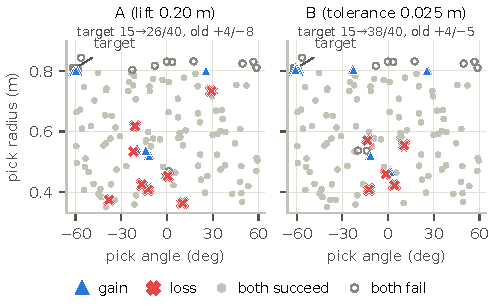
\includegraphics[width=\columnwidth]{fig_audit_map}
\caption{Paired audit outcomes by pick angle and radius. Each marker is one scene. Losses (red) lie in the workspace interior, far from the repaired boundary target (box at upper left). Most scenes that both controllers fail lie beyond 0.80\,m.}
\label{fig:map}
\end{figure}

\begin{table}[t]
\centering
\small
\setlength{\tabcolsep}{1.9pt}
\begin{tabular}{lcccccc}
\toprule
 & Target & Old & \multicolumn{2}{c}{Old} & Cond.\ loss, \% & Useful \\
\cmidrule(lr){4-5}
 & /40 & /120 & gain & loss & [95\% CI] & agg./pres. \\
\midrule
Parent & 15 & 106 & -- & -- & -- & -- \\
A: lift 0.20\,m & 26 & 102 & 4 & 8 & 7.5 [3.9, 14.2] & no/no \\
B: tol.\ 0.025\,m & 38 & 105 & 4 & 5 & 4.7 [2.0, 10.6] & no/no \\
\bottomrule
\end{tabular}
\caption{Frozen audit: 40 target and 120 old scenes, one reset each, paired against the parent. Conditional loss is losses divided by parent old successes, with a Wilson interval over scenes for this single context. Usefulness follows the objectives declared before the audit.}
\label{tab:audit}
\end{table}

\begin{table}[t]
\centering
\small
\setlength{\tabcolsep}{2.6pt}
\begin{tabular}{lcccccccc}
\toprule
 & \multicolumn{2}{c}{Committed} & & \multicolumn{3}{c}{Delivered (audit)} & \multicolumn{2}{c}{P(admit)} \\
\cmidrule(lr){2-3}\cmidrule(lr){5-7}\cmidrule(lr){8-9}
Gate & A & B & Deliv. & Tgt & Old & Loss & A & B \\
\midrule
Frozen & -- & -- & parent & 15 & 106 & 0 & -- & -- \\
Target-only & admit & admit & B & 38 & 105 & 5 & 0.99 & 1.00 \\
Aggregate & reject & reject & parent & 15 & 106 & 0 & 0.47 & 0.74 \\
Preservation & reject & reject & parent & 15 & 106 & 0 & 0.41 & 0.68 \\
\bottomrule
\end{tabular}
\caption{Gate decisions committed from the 24-rollout validation draw before the audit ran, and the delivered controller's audit outcomes (target /40, old /120). P(admit) is a diagnostic: the admission rate over 5{,}000 validation-sized draws resampled from the audit pools.}
\label{tab:gates}
\end{table}


\paragraph{Target neighborhood.} Table~\ref{tab:audit} gives the audit outcomes. The parent already succeeds on 15/40 target-neighborhood scenes, all at radius below 0.80\,m. Its 25 failures split into 11 lift stalls and 14 approach timeouts, a mode the development target never showed. A repairs every lift stall but no approach timeout, reaching 26/40. B's tolerance applies to all motion phases. It repairs all 11 lift stalls and 12 of the 14 approach timeouts; the remaining two get past the approach and then stall in the lift. B reaches 38/40. How far a repair generalizes depends on its mechanism, which three development resets of one scene could not reveal.

\paragraph{Old scenes.} The parent solves 106/120 old scenes; 9 of its 14 failures are approach timeouts beyond 0.80\,m, of which B fixes one and A none. A loses 8 old successes and gains 4, for a net change of $-4$; B loses 5 and gains 4, for a net change of $-1$. The losses lie in the interior, at radii from 0.36 to 0.73\,m (Figure~\ref{fig:map}). All are placement regressions: the parent's errors of 1.3--3.0\,cm become 3.0--4.7\,cm. Unlike in development, they do not vanish at a 4\,cm tolerance, where 2 and 3 losses remain. Neither candidate is useful under the aggregate or the zero-loss objective. B is useful under the 5\% tolerance.

\paragraph{Gates.} In the committed validation draw, each candidate lost one of eight old scenes and gained none (Table~\ref{tab:gates}). Aggregate and preservation therefore both rejected both candidates and kept the parent. Target-only admitted both and delivered B, trading 23 target gains for 5 old losses and 4 old gains. When validation-sized draws are resampled from the audit pools, aggregate and preservation disagree in only 6.4\% (A) and 5.8\% (B) of draws, while target-only admits in at least 99\%.

\paragraph{Why the compensation disappeared.} The development panel was dominated by the boundary ring: 9 of its 24 old scenes lay at 0.80\,m or beyond, four of them sharing the target's lift stall, whereas uniform sampling of the same region places only 10 of 120 old scenes there. A regression panel assembled around the failure being repaired over-represents that failure's family and inflates compensating gains. That is exactly the condition under which aggregate admission tolerates losses.

\section{Post-hoc Extension: A Candidate Population}
\paragraph{Design.} After the audit results were known, we froze and hashed a second protocol to ask whether its patterns hold beyond two candidates. It adds 24 edits drawn with a fixed seed from the same interface, each changing one or two parameters to values drawn uniformly within their bounds. They form a non-agent proposal distribution, not tuned to the target, and say nothing about proposer quality. A and B are re-tested unchanged on fresh validation (12 target, 8 old) and audit (30 target, 90 old) draws from the same populations, using the unchanged gate and analysis scripts. Gate decisions were committed before the first audit rollout. All 3{,}800 rollouts completed without retries, and the parent repeat again reproduced all 20 outcomes.

\begin{figure}[t]
\centering
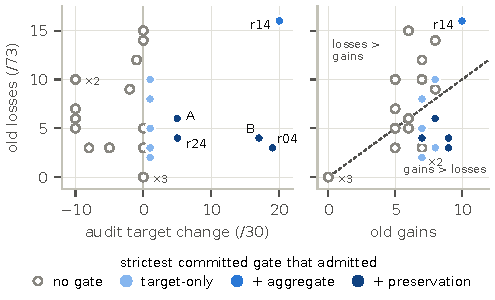
\includegraphics[width=\columnwidth]{fig_population}
\caption{Post-hoc extension, one marker per candidate. Left: audit target change against old losses; no target-improving candidate sits at zero losses. Right: old gains against old losses; below the dashed line, gains outnumber losses. Shading marks the strictest committed gate that admitted the candidate.}
\label{fig:population}
\end{figure}

\begin{table}[t]
\centering
\small
\setlength{\tabcolsep}{3.0pt}
\begin{tabular}{lcccccc}
\toprule
 & \multicolumn{3}{c}{Admitted} & \multicolumn{2}{c}{Agg.-useful} & \\
\cmidrule(lr){2-4}\cmidrule(lr){5-6}
Gate & /26 & w/ loss & losses & adm. & missed & Deliv. \\
\midrule
Target-only & 10 & 10 & 61 & 7 & 0 & B \\
Aggregate & 5 & 5 & 33 & 4 & 3 & B \\
Preservation & 4 & 4 & 17 & 4 & 3 & B \\
\bottomrule
\end{tabular}
\caption{Post-hoc extension: committed gate decisions over 26 candidates (A, B and 24 seeded random edits), scored on a fresh audit of 30 target and 90 old scenes. Losses are summed over admitted candidates. Under the aggregate objective 7 candidates are useful; under the zero-loss objective, none.}
\label{tab:population}
\end{table}


\paragraph{Every target improvement lost old successes.} Ten of the 26 candidates improve the target neighborhood, and all ten lose some of the parent's 73 old successes (10/10; Wilson 95\% interval 72--100\%). Their 61 losses are all placement regressions at radii below 0.80\,m. No candidate is useful under the zero-loss objective, and seven are useful under the aggregate objective. Gains and losses usually co-occur: 23 candidates have both, and 13 gain at least as many old scenes as they lose (Figure~\ref{fig:population}). The three edits that change only the grasp tolerance reproduce the parent on all 120 scenes.

\paragraph{Gates.} Target-only admitted exactly the ten target improvers, which carry 61 old losses (Table~\ref{tab:population}). Aggregate admitted five and preservation four, and every admitted candidate had audit losses: 33 and 17 in total. The stricter gates rejected three aggregate-useful candidates, each with a one-scene target gain. The two rules disagree in committed decisions only on r14, which fixes all 30 target scenes but loses 16 old successes for a net old change of $-6$: aggregate admitted it and preservation did not. Over resampled validation draws they disagree in 29\% of draws for r14 and 3\% on average. All three gates delivered B.

\paragraph{A and B on a new draw.} Their target gains replicate (from 10/30 to 15/30 and 27/30), and so does the conditional loss: 8.2\% and 5.5\%, against 7.5\% and 4.7\% in the first audit. The sign of the old net change does not. A and B now gain 8 and 7 old scenes against 6 and 4 losses, for net changes of $+2$ and $+3$, which makes both useful under the aggregate objective. Most of these gains are interior parent failures that settle just outside the 3\,cm tolerance, with parent errors of 3.0--4.5\,cm. This draw contains 8 such scenes among 90 old scenes, while the first audit had 4 among 120. The same placement perturbation that breaks some interior scenes rescues others, and the net balance depends on how many near-threshold failures the panel happens to contain.

\section{Discussion and Limitations}
Three observations follow, each specific to this case.
\begin{itemize}
\item Aggregate success hides losses only when gains offset them, and whether they do depends on the old panel. Panels inherited from failure discovery can manufacture the offset, and two uniform draws of the same region gave opposite net signs for the same repairs, while their conditional loss rates agreed.
\item At a 12-pair budget, aggregate and zero-loss admission rarely disagree: across 26 candidates they disagreed once, on the most harmful admitted edit. Stricter gates cut admitted losses from 61 to 33 to 17, but none admitted a loss-free improvement, because none existed.
\item Whether B should be deployed has no evidence-only answer. Across the two audits it added 23 and 17 target successes and lost 5 and 4 old successes, for net old changes of $-1$ and $+3$. The tolerance for loss, and the placement precision the deployment needs, must be declared before such evidence is read.
\end{itemize}

The study is narrow: one robot, one task and one repair context. The two repairs were proposed interactively, and the population extension, designed after the audit, uses random edits rather than an agent. The study makes no claim about agent competence, how common regressions are for real agent edits, or which gate is better in general. Intervals reflect sampling over scenes and candidates for this context only. Scripted parameter edits are not learned-policy updates, and simulation says nothing about physical safety. The failure was found by adaptive search near the workspace boundary. A broader study needs many repair contexts, a frozen sampled proposer with resampling baselines, and several tasks.

\paragraph{Reproducibility.} An anonymized artifact contains the runner, scene manifests, every rollout record, frozen hashes and the scripts that regenerate all tables and figures.

\bibliography{refs}

\end{document}
